%%%%%%%%%%%%%%%%%%%%%%%%%%%%%%%%%%%%%%%%%%%%%%%%%%%%%%%%%%%%%%%%%%%
%%% Documento LaTeX 																						%%%
%%%%%%%%%%%%%%%%%%%%%%%%%%%%%%%%%%%%%%%%%%%%%%%%%%%%%%%%%%%%%%%%%%%
% Título:		Capítulo 3
% Autor:  	Ignacio Moreno Doblas
% Fecha:  	2014-02-01, actualizado 2019-11-11
% Versión:	0.5.0
%%%%%%%%%%%%%%%%%%%%%%%%%%%%%%%%%%%%%%%%%%%%%%%%%%%%%%%%%%%%%%%%%%%
% !TEX root = A0.MiTFG.tex

\section{Segunda iteración: Funcionalidad básica}
    \subsection{Resumen}
        La segunda iteración gira en torno a la creación de un primer prototipo funcional que realice, aunque de forma parcial y poco intuitiva, las funciones deseadas para el producto final.

        Centrarse únicamente en la funcionalidad a esta altura del proyecto favorece a reducir el tiempo invertido en pulir detalles que no son realmente necesarios en esta fase tan temprana, economizando el tiempo de desarrollo.

    \subsection{Requisitos}
        Los requisitos a realizar en esta iteración son el 1.3.1, el 1.3.2, el 1.3.5 y el 2.3 de la tabla de requisitos iniciales (Tabla \ref{tab:Requisitos}). Además, derivado de la iteración anterior, se va a implementar el requisito 1.5 de la tabla completa. \ref{tab:RequisitosFinales}. Estos requisitos dan lugar a las siguientes tareas:
    
        \begin{enumerate}
            \item Implementar un mecanismo por el que seleccionar el fichero de entrada.
            \item Implementar la interfaz para los algoritmos de detección.
            \begin{enumerate}
                \item Almacenar la señal de entrada en un buffer.
                \item Definir la interfaz
                \item Implementar un algoritmo simple de detección.
            \end{enumerate}
            \item Mostrar los resultados del análisis en el panel de usuario.
        \end{enumerate}
        
    \subsection{Desarrollo}
        
        La primera tarea, \textit{seleccionar la entrada de datos}, se ha resuelto mediante el empleo de un "QListView" \cite{QListView} al que se le ha configurado una carpeta raíz donde se colocarán todos los ficheros de datos junto con unos filtros para que solo muestre estos. Haciendo uso del SLOT \char`_clicked se puede obtener la ruta al fichero que clickea el usuario dentro del widget, permitiendo pasarla como parámetro a la función de lectura implementada en la anterior iteración. 
        
        \begin{figure}[H] 
                \centering
                        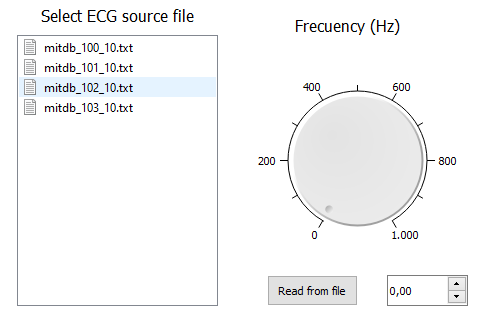
\includegraphics[width = 0.8 \linewidth]{figuras/fileView.png}
                \caption{Estado de la configuración en el panel de control tras la finalización de la segunda iteración.}
                \label{fig:fileView}
        \end{figure}
        
        Para el \textit{almacenamiento de la señal} se ha implementado un buffer circular empleando una estructura que contiene un array de tipo int32 de 1024 posiciones y una variable para indicar el índice 0 relativo llamada “Head”, una vez inicializado este índice apunta al espacio de memoria donde está almacenado el dato más reciente. Además se proveen dos funciones auxiliares encargadas de introducir y leer elementos del buffer respecto a la posición de la variable Head. 
        
        La función encargada de introducir nuevas muestras modifica el Head del buffer para mantener el estado actualizado, su funcionamiento se explica en el diagrama \ref{fig:bufferDiagramAppend}. 
    
        \begin{figure}[H] 
                \centering
                        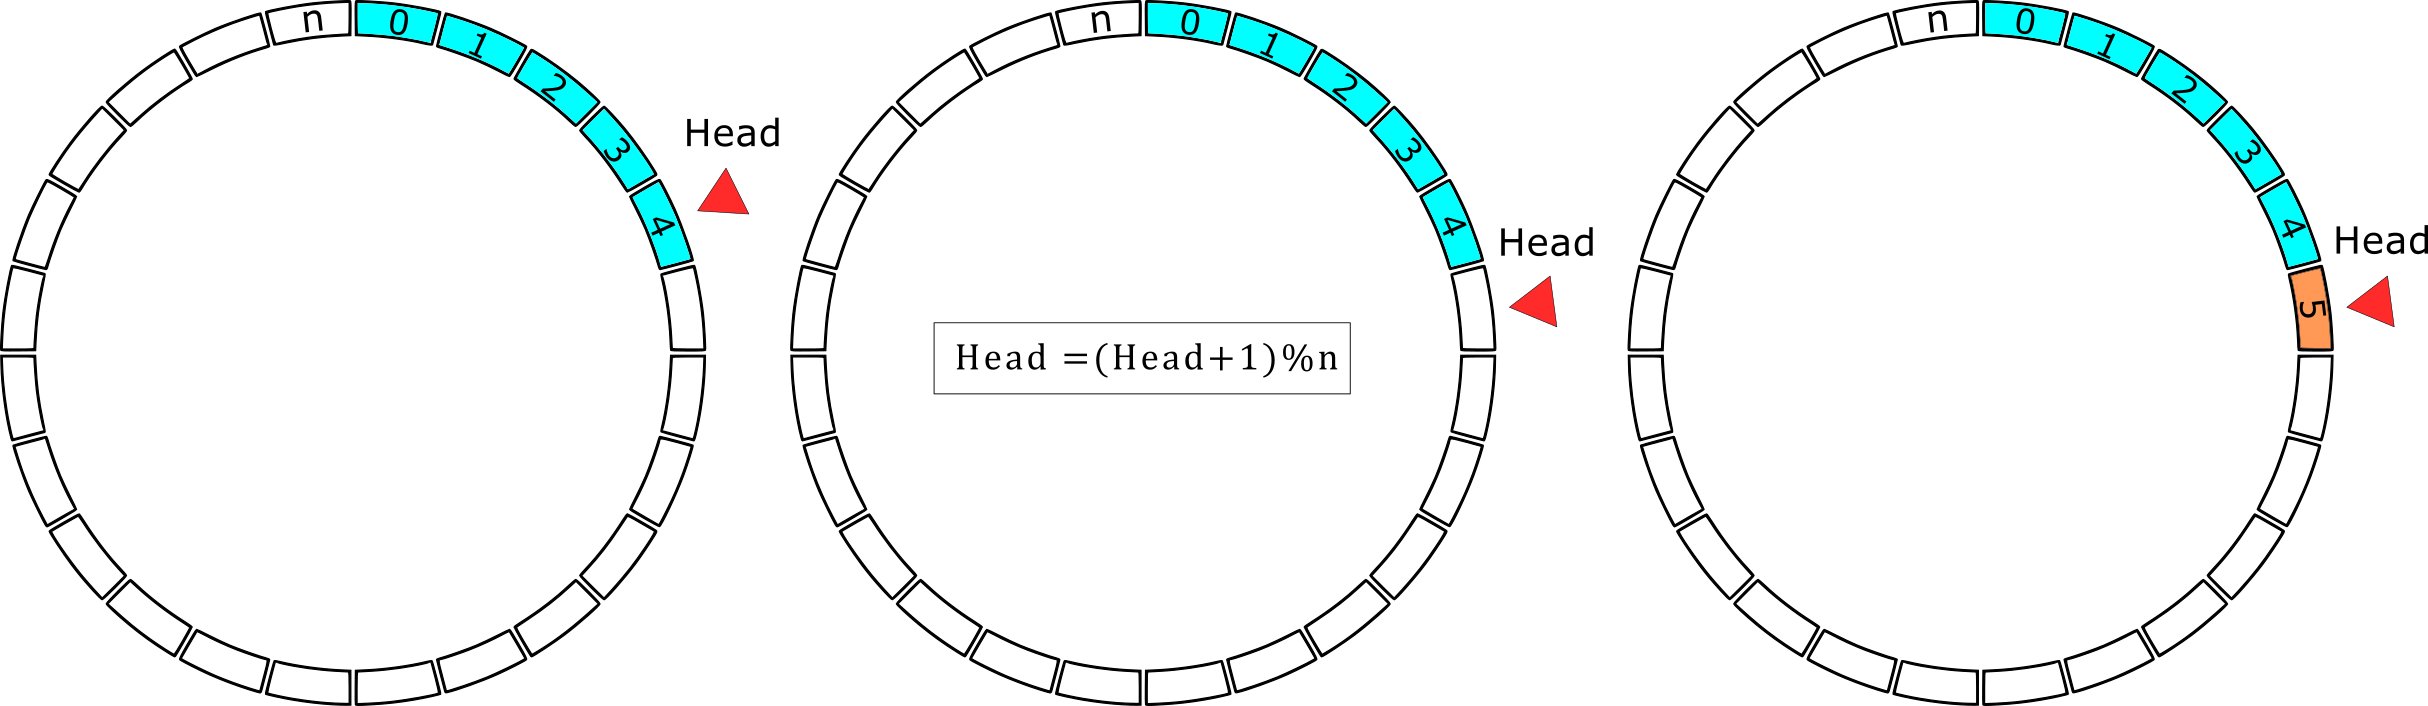
\includegraphics[width = \linewidth]{figuras/bufferAppend.png}
                \caption{Funcionamiento de \char`"AppendSample", función encargada de introducir muestras en el buffer.}
                \label{fig:bufferDiagramAppend}
        \end{figure}
        
        La función encargada de extraer las muestras simplemente recorre el array de forma relativa a la posición del Head como si se tratara de un array normal, retirando del usuario la necesidad de controlar los límites de este. Su funcionamiento está explicado en el diagrama \ref{fig:bufferDiagramGet}.
        
        \begin{figure}[H]
                \centering
                        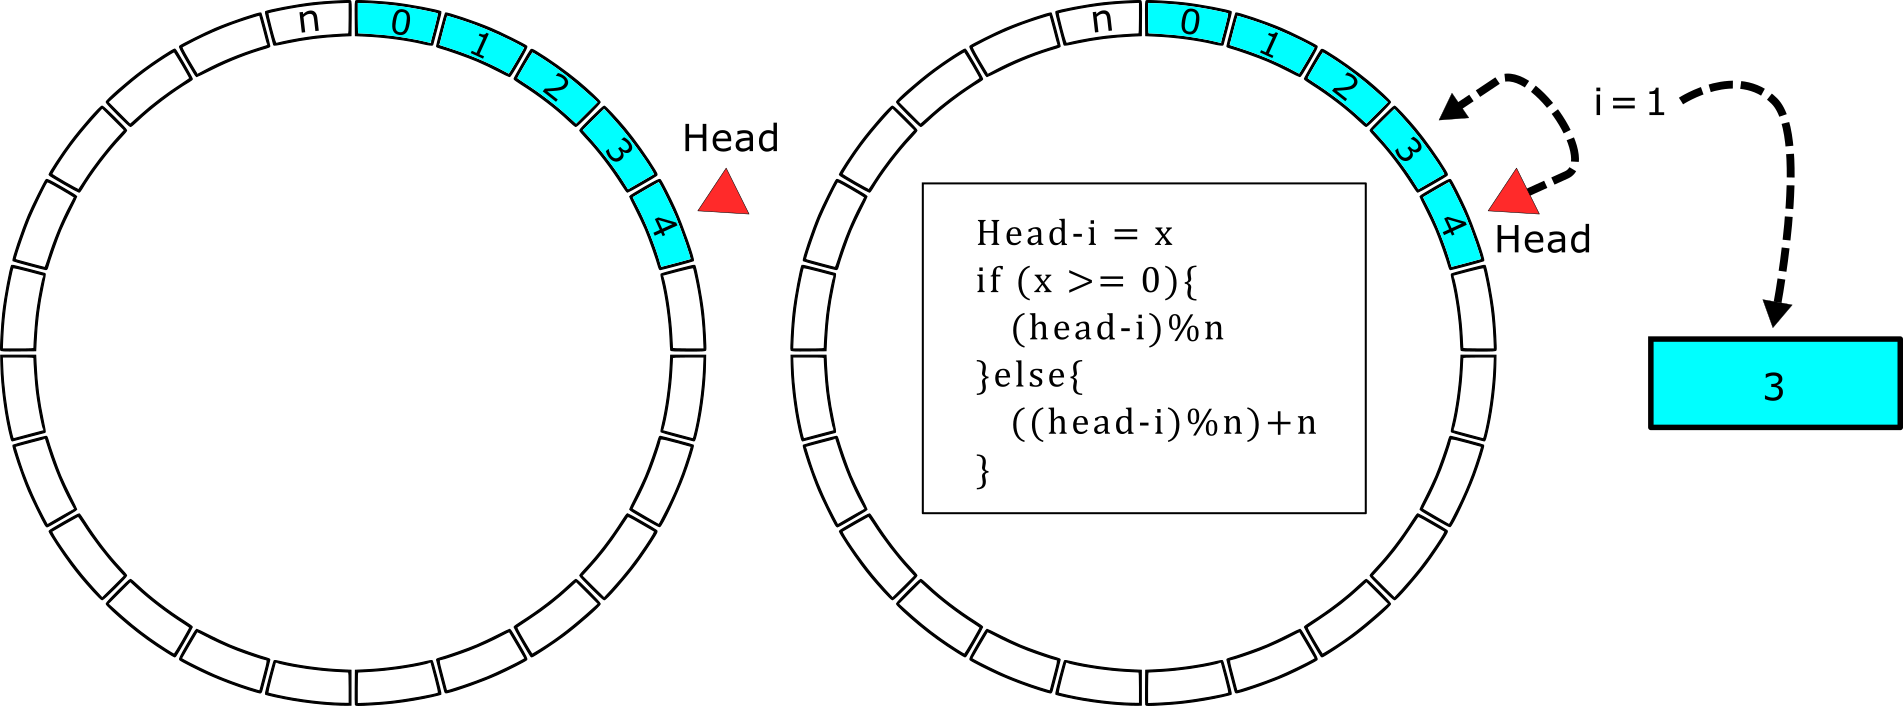
\includegraphics[width = 0.9 \linewidth]{figuras/bufferGet.png}
                \caption{Funcionamiento de "GetSample", función en cargada de extraer las muestras del buffer.}
                \label{fig:bufferDiagramGet}
        \end{figure}
        
        Respecto a la tarea 2.b, si bien no es posible generar una Interfaz propiamente dicha por ser un concepto procedente de la programación orientada a objetos, lo que se trata de lograr es limitar todas las modificaciones que deberá hacer un futuro usuario para introducir su algoritmo a un solo fichero, evitando la necesidad de modificar las llamadas a las funciones en otros ficheros de código. 

        La implementación se ha realizado mediante punteros a funciones. Se ha definido un tipo correspondiente a un puntero a una función con la firma establecida. De esta forma el usuario puede asignar al puntero cualquier función que desarrolle mientras satisfaga la firma impuesta por el mismo, haciendo las veces de interfaz.
        
        En el extracto \ref{code:interface} puede observarse de forma compacta la implementación del funcionamiento previamente descrito. Como se observa la función espera como entrada un puntero al buffer circular y tiene como salida una estructura de tipo PARAMETERS\char`_ECG\char`_PROCESSED, que corresponde con el modelo que espera el panel de usuario en el paquete. Esta estructura contiene un array para almacenar la ubicación de los picos detectados, un array para almacenar los valores de esos picos, un parámetro opcional para incluir un threshold y otro parámetro para anotar la cantidad de picos detectados.
        
        \code{Abstracto de la interfaz para el algoritmo del usuario.}{code/interface.cpp}{code:interface}{C++}
        
        A pesar de no ser estrictamente necesario si que resulta interesante \textit{implementar un algoritmo de detección} simplificado, pues en iteraciones posteriores será necesario para testear y además hace las pruebas en general más intuitivas. Para no añadir más complejidad de la necesaria se ha optado por un sencillo algoritmo que comprueba para cada muestra si se trata de un máximo local y si su valor está por encima de cierto umbral. Si se dan las dos condiciones entonces se asume que se trata de un pico R en la señal ECG, y por lo tanto, una pulsación. El código puede verse en el extracto \ref{code:BasicAlg}.
        
        \code{Algoritmo de detección de picos R sencillo}{code/BasicAlgorithm.c}{code:BasicAlg}{C++}
        

        Para la tercera tarea se han decidido implementar varios mecanismos para \textit{mostrar los resultados al usuario}. Se ha añadido una gráfica empleando el widget QwtPlot donde se muestra la señal ECG leída del fichero en tiempo real. Sobre ella se dibujan los picos R detectados por el algoritmo. Además se ofrece la posibilidad de dibujar el threshold de detección si el algoritmo emplea uno y un recuadro donde se muestra el valor de la tasa cardíaca instantánea medida. En la figura \ref{fig:resultsBasic} puede observarse el formato de salida.

        \begin{figure}[H]
                \centering
                        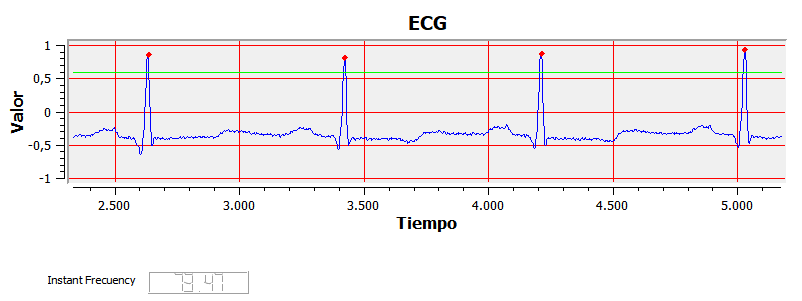
\includegraphics[width =\linewidth]{figuras/ResultsBasic.png}
                \caption{Gráfica que muestra los resultados del análisis llevado a cabo por el algoritmo.}
                \label{fig:resultsBasic}
        \end{figure}
        
    \subsection{Pruebas}
        
        La prueba de la tarea 1 de esta iteración se ha realizado simplemente proveyendo al programa con dos ficheros diferente y mediante el selector leer sus frecuencias. Puesto que la lectura de la frecuencia desde un fichero estaba testeada desde la iteración anterior, esto es suficiente para probar el funcionamiento del selector de ficheros.La figura \ref{fig:fileSelectorTest} se adjunta como prueba del test.

        \begin{figure}[H]
                \centering
                        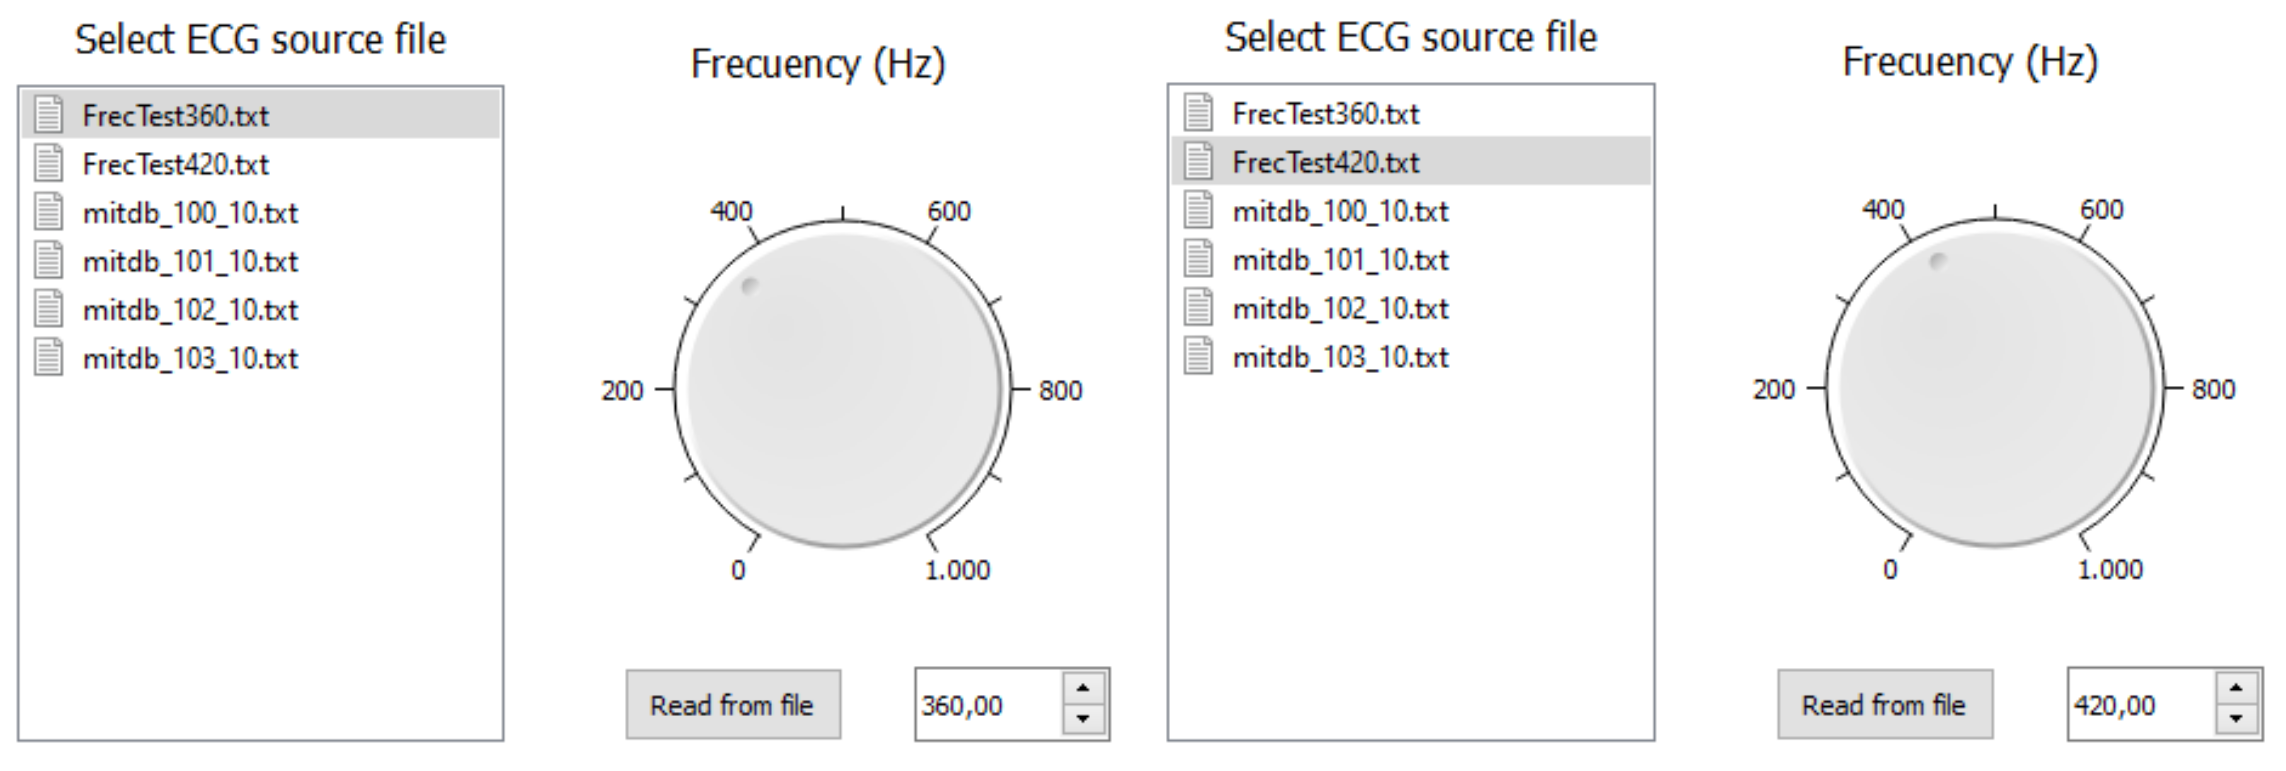
\includegraphics[width = \linewidth]{figuras/FileSelectorTest.png}
                \caption{Lectura de diferentes ficheros desde el selector.}
                \label{fig:fileSelectorTest}
        \end{figure}

        \clearpage
        Como prueba para el buffer circular se han implementado dos tests unitarios en QT. Como la implementación del buffer es idéntica si este funciona correctamente en QT no es necesario testearlo en la TIVA. Los casos implementados son ``BufferStorage'' y ``BufferCircularity'': 
        
        \begin{itemize}
            \item El primero de ellos comprueba que los datos son almacenados y leídos correctamente, asignando al buffer valores conocidos y comprobando cada uno de ellos. 
            \item La segunda prueba funciona de forma similar, solo que esta vez se han introducido en el buffer más elementos que su longitud total, esto debería sobre escribir los datos más antiguos. Al emplear unos datos de entrada sencillos, la sobre escritura es predecible, y por tanto, comprobable.
        \end{itemize}
        
         El código de ambas pruebas puede ser comprobado en el extracto \ref{code:TestBuffer}.

        Para testear la interfaz, o mejor dicho, el puntero a una función simplemente se ha ejecutado el código en modo debug y comprobado que en el momento apropiado este ejecutaba la función correctamente mediante un punto de ruptura. 

        El test correspondiente al envío de los resultados de vuelta al panel resulta ser más sencillo de lo que pueda parecer a priori. Pues el envío correcto de los datos no implica que los datos sean correctos, por lo que no es necesario tener de momento un algoritmo capaz de detectar eficazmente la tasa cardiaca. Comprobando mediante puntos de ruptura que el dato enviado y recibido son el mismo. 
        
        Aprovechando que ya se dispone de una entrada de datos procedente del dispositivo, se puede probar también que la gráfica pinta correctamente los datos, para esto solo hay que asegurar que los datos de entrada son almacenados bien en el buffer de la gráfica empleando algunos puntos de ruptura y el inspector de variables del modo debug. El proceso de pintado en sí mismo es llevado acabo con una librería de QT por lo que no necesita de prueba.
        
        \code{Código de los tests unitarios del buffer circular}{code/TestBuffer.c}{code:TestBuffer}{C++}

        
    \subsection{Conclusiones}
    
        Con la finalización de esta iteración queda definida la funcionalidad general, sin embargo para gozar de un primer prototipo cerrado es necesario llevar a cabo algunos cambios en el futuro cercano.
        
        Actualmente la interfaz para el algoritmo se ejecuta dentro de la rutina de recepción de los mensajes. Aunque es capaz de llevar a cabo todas la funciones que se le requieren sería más óptimo separar el procesado de la señal en una tarea aparte gestionada por el sistema operativo. Con esto se conseguiría además aislarla para simplificar la medida del rendimiento, permitiendo además emplear los propios mecanismos de FreeRTOS \cite{FreeRTOS} para realizar las medidas de rendimiento necesarias.
        
        Esta modificación se incluye como requisito en la tabla de final (\ref{tab:RequisitosFinales}) con el código: 2.5, aislamiento del procesado de señal.